% Noise Padifier - manuel d'utilisation.
% pdflatex manuel.tex (trois passes) ; figures : python3 figures.py (doc/fig_*.pdf).
% Copyright (C) 2026 Padifier authors - SPDX-License-Identifier: GPL-3.0-or-later
\documentclass[a4paper,11pt]{article}
\usepackage[T1]{fontenc}
\usepackage[utf8]{inputenc}
\usepackage[french]{babel}
\usepackage{lmodern}
\usepackage{microtype}
\usepackage[margin=2.3cm]{geometry}
\usepackage{amsmath,amssymb}
\usepackage{graphicx}
\usepackage{booktabs}
\usepackage{array}
\usepackage{tabularx}
\usepackage{xcolor}
\usepackage{tikz}
\usetikzlibrary{arrows.meta,positioning,fit,calc}
\usepackage{enumitem}
\usepackage[hidelinks]{hyperref}

\definecolor{amber}{HTML}{96691A}
\definecolor{violet}{HTML}{6246AA}
\definecolor{ink}{HTML}{26203A}
\definecolor{paper}{HTML}{F4F2F8}

\newcommand{\ctl}[1]{\textsf{\textbf{#1}}}   % nom d'un élément de l'interface
\newcommand{\dB}{\,dB}
\newcommand{\dBFS}{\,dBFS}
\setlist{itemsep=1pt,topsep=3pt}
\emergencystretch=3em
\graphicspath{{./}{captures/}}

\title{\textsf{NOISE} \textcolor{violet}{\textbf{PADIFIER}}\\[4pt]
\large Manuel d'utilisation et description de l'algorithme}
\author{Version 1.1.0}
\date{}

\begin{document}
\maketitle

\begin{center}
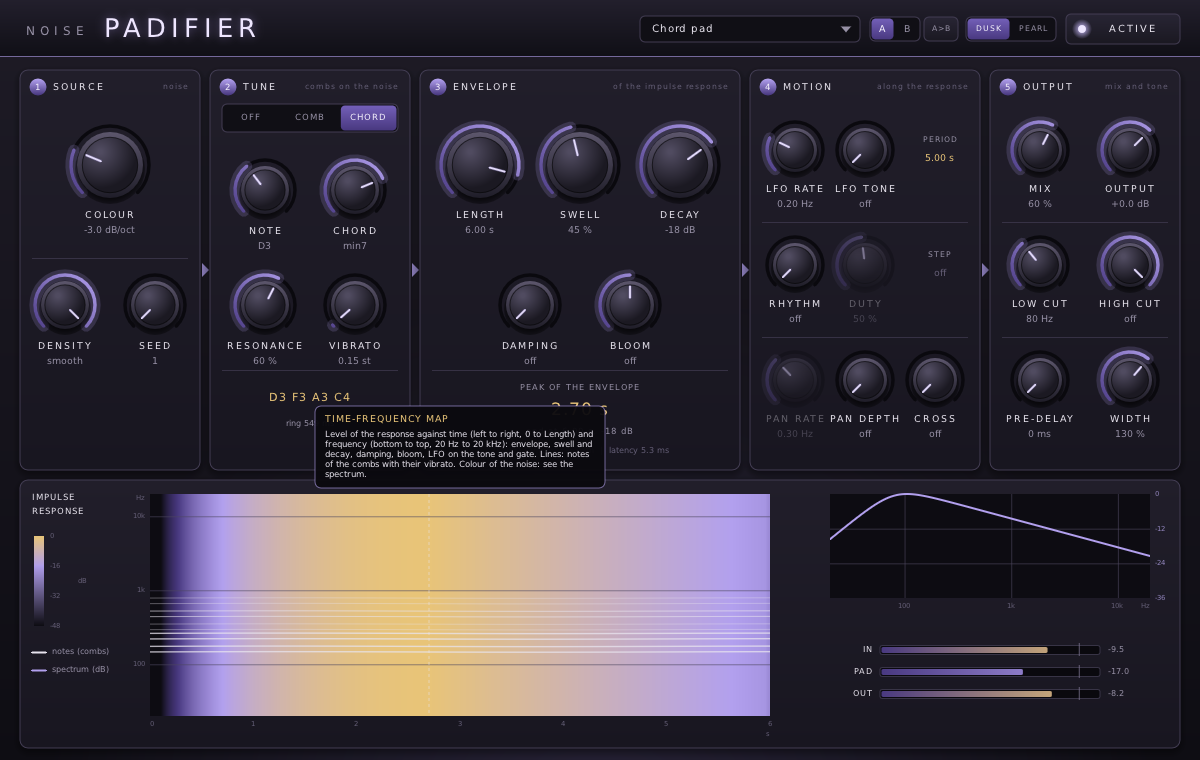
\includegraphics[width=0.92\textwidth]{capture_dusk.png}
\end{center}

\newpage
\tableofcontents
\newpage

% ==============================================================================================
\section{Présentation}

Noise Padifier transforme n'importe quel son en nappe (\emph{pad}). Le signal est convolué avec
une réponse impulsionnelle faite de \textbf{bruit} sous une \textbf{enveloppe} réglable, longue
de 0,1 à 10\,s : chaque note, chaque attaque, est étalée sur toute la durée de cette réponse.
Comme le bruit contient toutes les fréquences, le timbre de la source est gardé (ses harmoniques
restent à leur place) mais son évolution dans le temps disparaît : une note brève devient un son
tenu qui monte puis s'éteint selon l'enveloppe (figure~\ref{fig:pad}).

Le bruit lui-même se façonne : sa couleur (du brun au violet), sa densité (du bruit lisse à un
nuage de grains), un accord sur une note ou un accord par des filtres en peigne, une enveloppe
qui dépend de la fréquence (les aigus qui meurent plus tôt, les graves qui s'épanouissent plus
tard), un LFO, un rythme calé sur le tempo, un mouvement stéréo et une vraie stéréo croisée.
Tous ces traitements agissent \textbf{le long de la réponse} : ils sont calculés une fois, quand
la réponse est construite, et ne coûtent rien pendant la lecture.

\begin{figure}[htbp]
\centering
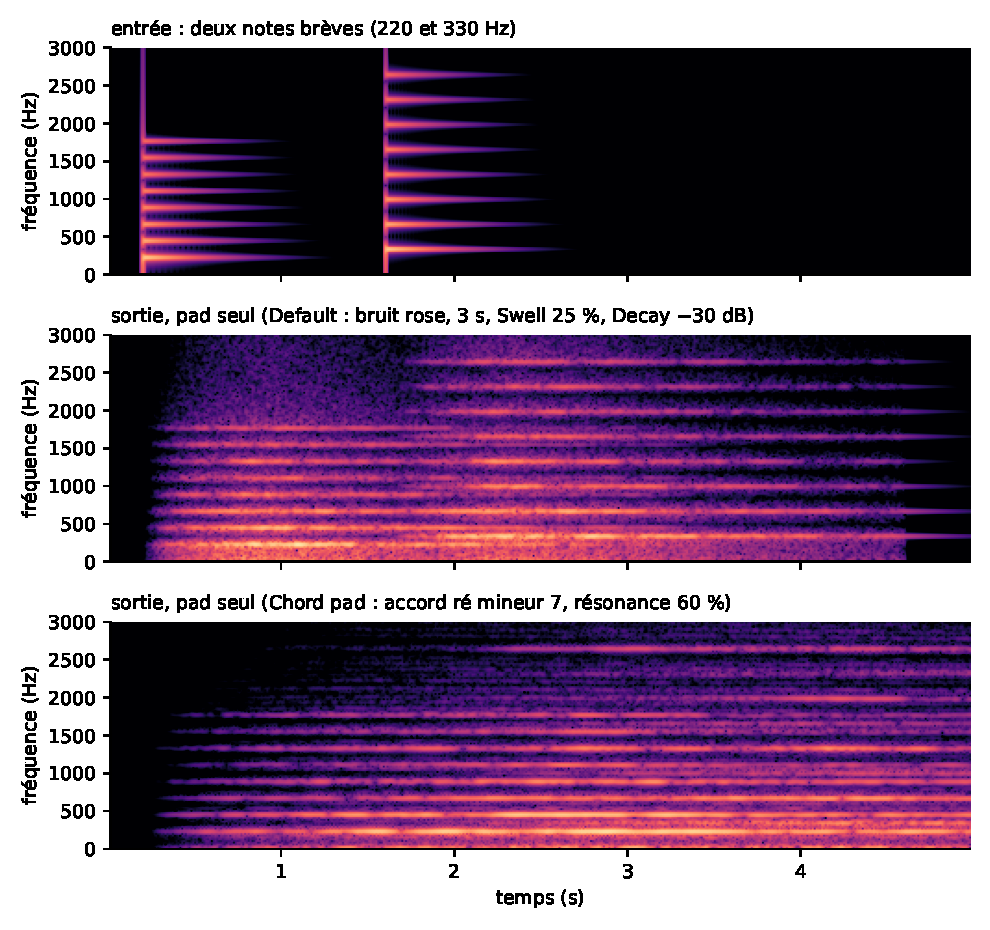
\includegraphics[width=\textwidth]{fig_pad.pdf}
\caption{Deux notes brèves (en haut), ce qu'en fait le préréglage Default (au milieu : chaque
note dure 3\,s, monte en 0,75\,s puis décroît), et le préréglage Chord pad (en bas : la nappe est
accordée sur un accord de ré mineur 7).}
\label{fig:pad}
\end{figure}

Autour de la convolution : pré-retard, coupe-bas et coupe-haut sur le pad, largeur stéréo, mélange
avec le son sec, gain de sortie, préréglages, comparaison A/B.

\paragraph{Formats.} VST3 et CLAP pour Windows 64 bits ; VST3, CLAP et LV2 pour Linux. Le greffon
est stéréo (deux entrées, deux sorties). Sa \textbf{latence est de 256 échantillons} (5,3\,ms à
48\,kHz), déclarée à l'hôte, qui la compense.

\paragraph{Licence.} GPL 3 ou ultérieure (fichier \texttt{COPYING}). L'interface et l'adaptation
aux formats reposent sur DPF (licence ISC) ; les transformées de Fourier sur pffft de Julien
Pommier (licence de FFTPACK, de type BSD).

% ==============================================================================================
\section{Installation}

\paragraph{Windows.} Lancer l'installateur \texttt{Noise-Padifier-1.1.0-setup.exe}. Il installe
le VST3 (obligatoire) et, si on le coche, le CLAP et les manuels (français et anglais), puis
ajoute un désinstalleur (\og Programmes et fonctionnalités\fg). À la main, copier :
\begin{itemize}
\item le dossier \texttt{noise\_padifier.vst3} dans \verb|C:\Program Files\Common Files\VST3\| ;
\item \texttt{noise\_padifier.clap} dans \verb|C:\Program Files\Common Files\CLAP\|.
\end{itemize}

\paragraph{Linux.} Copier \texttt{noise\_padifier.vst3} dans \verb|~/.vst3/|,
\texttt{noise\_padifier.clap} dans \verb|~/.clap/| ou \texttt{noise\_padifier.lv2} dans
\verb|~/.lv2/|.

Relancer ensuite l'analyse des greffons de l'hôte. Le désinstalleur laisse les préférences et
les préréglages de l'utilisateur (section~\ref{sec:fichiers}).

% ==============================================================================================
\section{Prise en main en une minute}

\begin{enumerate}
\item \textbf{En insert} sur une piste : le préréglage \ctl{Default} est chargé (bruit rose,
  3\,s, Mix 50\,\%). \textbf{En départ auxiliaire} : choisir \ctl{Send (100 \% wet)}, qui ne rend
  que le pad.
\item Régler la durée de la nappe avec \ctl{LENGTH}, sa montée avec \ctl{SWELL} et sa fin avec
  \ctl{DECAY} ; la carte en bas montre la réponse obtenue.
\item Choisir la couleur avec \ctl{COLOUR} : vers la gauche plus sombre et chaud, vers la droite
  plus brillant ; affiner avec \ctl{LOW CUT} et \ctl{HIGH CUT}.
\item Pour une nappe accordée : \ctl{TUNE} sur \ctl{COMB} (une note) ou \ctl{CHORD} (un accord),
  puis \ctl{NOTE}, \ctl{CHORD} et \ctl{RESONANCE}.
\item Pour du mouvement : \ctl{RHYTHM} (pulsation sur le tempo), \ctl{PAN DEPTH} (balancement
  stéréo), \ctl{VIBRATO} ou \ctl{LFO TONE}.
\item Doser avec \ctl{MIX}. Les préréglages montrent chaque traitement.
\end{enumerate}

\section{L'interface}

La fenêtre (1200 × 760 points, redimensionnable en gardant ses proportions, nette sur les écrans
à haute densité) se lit de gauche à droite dans l'ordre du signal : cinq sections numérotées
reliées par des flèches, puis, en bas, la carte de la réponse, le spectre du pad et les
vu-mètres. Chaque élément a une bulle d'aide au survol ; pour un bouton, son titre donne la valeur
détaillée. Un bouton sans effet avec les autres réglages est grisé (par exemple NOTE quand TUNE
est sur OFF) ; il reste utilisable.

\begin{center}
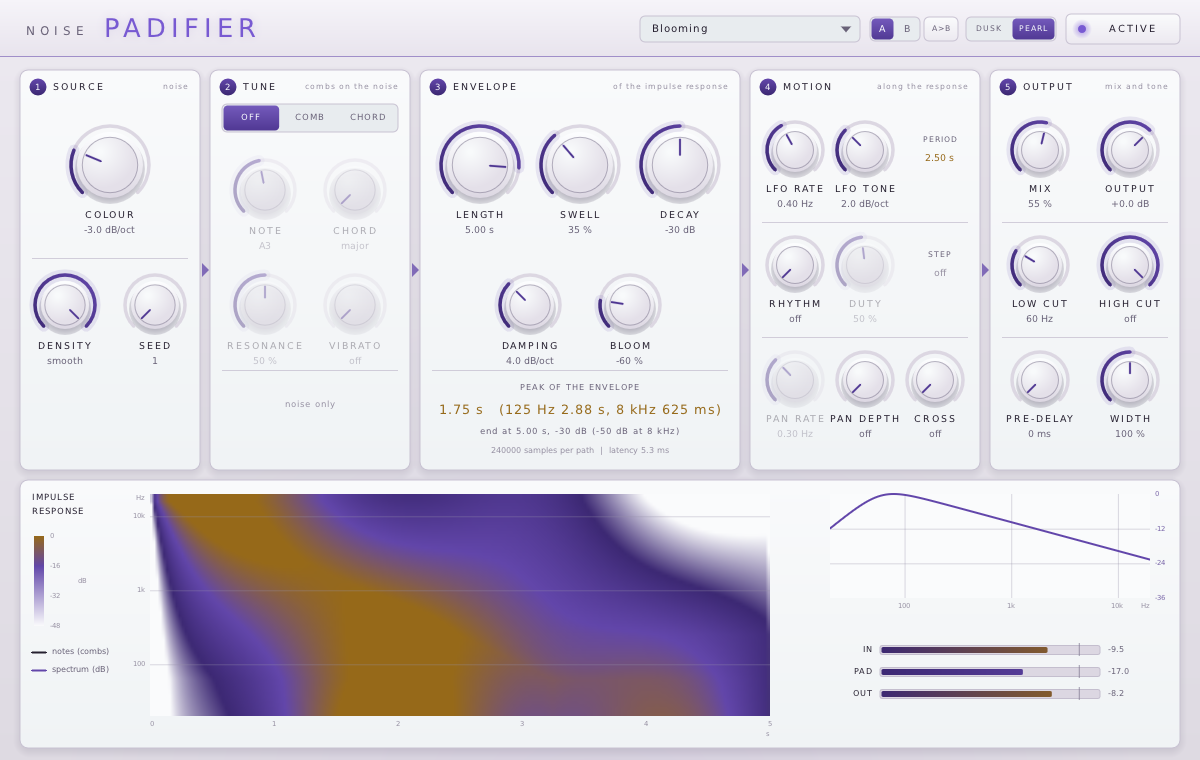
\includegraphics[width=0.85\textwidth]{capture_pearl.png}\\[2pt]
\small Thème clair \ctl{PEARL}, préréglage Blooming, bulle d'aide de BLOOM.
\end{center}

\subsection{En-tête}
\begin{description}
\item[Préréglages.] Liste déroulante : un clic l'ouvre ; elle montre les préréglages d'usine
  (\ctl{FACTORY}), un trait, vos préréglages (\ctl{USER}, par ordre alphabétique), un trait, puis
  \ctl{Save current settings\ldots}. Le préréglage courant est marqué d'un point ; \og *\fg{}
  après son nom signale un réglage modifié depuis son chargement. La molette sur la boîte fermée
  passe au préréglage suivant ou précédent. Détails en section~\ref{sec:prereglages}.
\item[A | B et A>B.] Deux jeux de réglages à comparer : un clic sur \ctl{A} ou \ctl{B} bascule
  (le jeu quitté est gardé, l'autre est rechargé ; à la première visite, B part d'une copie de
  A). \ctl{A>B} (ou \ctl{B>A}) copie le jeu courant dans l'autre. Les deux jeux sont
  enregistrés avec le projet.
\item[DUSK | PEARL.] Thème sombre ou clair, sans effet sur le son ; c'est une préférence de
  l'ordinateur, commune à toutes les instances et à tous les projets.
\item[ACTIVE / BYPASSED.] Le Bypass déclaré à l'hôte (section~\ref{sec:lissage}).
\end{description}

\subsection{Section 1 : SOURCE}
\ctl{COLOUR}, \ctl{DENSITY} et \ctl{SEED} : le bruit de départ.

\subsection{Section 2 : TUNE}
Le sélecteur \ctl{OFF | COMB | CHORD}, puis \ctl{NOTE}, \ctl{CHORD}, \ctl{RESONANCE} et
\ctl{VIBRATO}. Au-dessous : la note et sa fréquence (ou les notes de l'accord) et le temps de
résonance des peignes.

\subsection{Section 3 : ENVELOPE}
\ctl{LENGTH}, \ctl{SWELL}, \ctl{DECAY}, \ctl{DAMPING} et \ctl{BLOOM}. Au-dessous : l'instant du pic
de l'enveloppe (à 125\,Hz et 8\,kHz quand Bloom est actif), la fin de la réponse et son niveau (et
à 8\,kHz avec Damping), le nombre d'échantillons par trajet et la latence.

\subsection{Section 4 : MOTION}
Trois rangées : le LFO (\ctl{LFO RATE}, \ctl{LFO TONE}, et sa période), le rythme (\ctl{RHYTHM},
\ctl{DUTY}, et la durée d'un pas au tempo de l'hôte), la stéréo (\ctl{PAN RATE}, \ctl{PAN DEPTH},
\ctl{CROSS}).

\subsection{Section 5 : OUTPUT}
\ctl{MIX}, \ctl{OUTPUT}, \ctl{LOW CUT}, \ctl{HIGH CUT}, \ctl{PRE-DELAY} et \ctl{WIDTH}.

\subsection{Carte, spectre et vu-mètres}
\begin{itemize}
\item à gauche, la \textbf{carte temps-fréquence} de la réponse : le temps de 0 à Length de gauche
  à droite, la fréquence de 20\,Hz à 20\,kHz de bas en haut, le niveau en couleur (de 0 à
  $-48$\dB, échelle à gauche). On y voit l'enveloppe, Damping, Bloom, LFO TONE et la porte de
  RHYTHM ; les traits clairs sont les notes des peignes (harmoniques en COMB, notes de l'accord et
  deux harmoniques en CHORD), avec leur vibrato ; en tirets, le pic de l'enveloppe. La couleur du
  bruit n'y figure pas : elle est sur le spectre ;
\item à droite, le \textbf{spectre du pad} : couleur du bruit et filtres, en dB, le point le plus
  haut à 0\dB ;
\item au-dessous, trois vu-mètres de crête : \ctl{IN} (entrée), \ctl{PAD} (pad seul, après les
  filtres et Width, avant le mélange), \ctl{OUT} (sortie), en dBFS ; après une crête, l'affichage
  redescend avec une constante de temps de 0,25\,s.
\end{itemize}

\subsection{Manipuler les boutons}
\begin{itemize}
\item glisser verticalement ; \textsf{Maj} pour un réglage fin ;
\item molette (\textsf{Maj} : fin) ;
\item double-clic ou \textsf{Ctrl}+clic : valeur par défaut ;
\item clic droit : saisie de la valeur au clavier (\textsf{Entrée} valide, \textsf{Échap}
  annule ; la virgule est acceptée comme séparateur décimal).
\end{itemize}

% ==============================================================================================
\section{Les réglages}

\begin{center}
\small
\begin{tabularx}{\textwidth}{@{}l l l X@{}}
\toprule
Réglage & Plage & Défaut & Rôle \\
\midrule
\multicolumn{4}{@{}l}{\textsf{1 SOURCE}} \\
Colour & $-6$--+6\dB/oct & $-3$ & pente du spectre du bruit ($-3$ : rose) \\
Density & 10--10\,000 /s & lisse & impulsions par seconde (au maximum : bruit lisse) \\
Seed & 1--99 & 1 & tirage du bruit \\
\multicolumn{4}{@{}l}{\textsf{2 TUNE}} \\
Tune & off, comb, chord & off & peigne sur la note, ou peignes sur un accord \\
Note & C1--C7 & A3 & note du peigne, fondamentale de l'accord \\
Chord & 9 accords & major & sorte d'accord \\
Resonance & 0--100\,\% & 50\,\% & temps de résonance des peignes (20\,ms à 5\,s) \\
Vibrato & 0--12 demi-tons & 0 & profondeur du LFO sur la note \\
\multicolumn{4}{@{}l}{\textsf{3 ENVELOPE}} \\
Length & 0,1--10\,s & 3\,s & longueur de la réponse \\
Swell & 0--100\,\% & 25\,\% & montée de l'enveloppe, en part de la longueur \\
Decay & $-60$--0\dB & $-30$\dB & niveau de l'enveloppe à la fin \\
Damping & 0--12\dB/oct & 0 & perte des aigus à la fin \\
Bloom & $-100$--+100\,\% & 0 & déplacement du pic avec la fréquence \\
\multicolumn{4}{@{}l}{\textsf{4 MOTION}} \\
LFO rate & 0,05--10\,Hz & 0,5\,Hz & vitesse du LFO (vibrato, couleur) \\
LFO tone & 0--6\dB/oct & 0 & profondeur du LFO sur la couleur \\
Rhythm & off, 1/1--1/32 & off & porte calée sur le tempo (pointées, triolets) \\
Duty & 5--100\,\% & 50\,\% & part ouverte de chaque pas \\
Pan rate & 0,05--10\,Hz & 0,3\,Hz & vitesse du mouvement stéréo \\
Pan depth & 0--100\,\% & 0 & profondeur du mouvement stéréo \\
Cross & 0--100\,\% & 0 & vraie stéréo : croisements gauche-droite \\
\multicolumn{4}{@{}l}{\textsf{5 OUTPUT}} \\
Mix & 0--100\,\% & 50\,\% & part du pad (puissance constante) \\
Output & $-24$--+12\dB & 0\dB & gain de toute la sortie \\
Low cut & 20\,Hz (off)--1\,kHz & off & passe-haut 12\dB/octave sur le pad \\
High cut & 1--20\,kHz (off) & off & passe-bas 12\dB/octave sur le pad \\
Pre-delay & 0--500\,ms & 0 & retard du pad \\
Width & 0--200\,\% & 100\,\% & largeur stéréo du pad \\
Bypass & oui/non & non & entrée non traitée (retardée), fondu de 10\,ms \\
\bottomrule
\end{tabularx}
\end{center}

\subsection{Source}

\paragraph{Colour.} Pente du spectre du bruit, en décibels par octave (de puissance) : $-6$, bruit
brun, sombre et grave ; $-3$, bruit rose (même énergie par octave), chaud et plein, proche de
l'équilibre d'une réverbération ; 0, bruit blanc, brillant et aérien, dont le souffle s'entend
davantage dans l'aigu ; $+3$ bleu et $+6$ violet, de plus en plus aigus. Figure~\ref{fig:spectre}.

\paragraph{Density.} Au maximum, le bruit est lisse (gaussien). En dessous, c'est un bruit épars
(\emph{velvet noise}) : une impulsion de signe aléatoire, placée au hasard, dans chaque intervalle
de 1/Density seconde. À quelques milliers par seconde, il reste lisse à l'oreille ; à quelques
dizaines, chaque son est répété en un nuage de grains ou d'échos distincts.

\paragraph{Seed.} Le bruit est tiré d'un générateur pseudo-aléatoire : chaque valeur de Seed donne
un autre bruit de même nature. Les différences sont de détail (le \og grain\fg, quelques fréquences
un peu plus ou un peu moins présentes) ; la même valeur donne toujours exactement la même réponse,
sur tout ordinateur.

\subsection{Tune}

\paragraph{Tune.} \ctl{OFF} : bruit seul. \ctl{COMB} : le bruit passe dans un filtre en peigne
accordé sur NOTE ; ses résonances sont les harmoniques de la note, et le pad prend la couleur d'une
corde ou d'un tuyau sur cette note. \ctl{CHORD} : un peigne par note de l'accord, additionnés. La
convolution ne crée pas de fréquence absente de l'entrée : le pad fait ressortir ce que la source
contient près de ces notes ; une source riche (bruit, percussion, accord dense) donne une nappe
nettement accordée, une note isolée éloignée de l'accord donne peu de son.

\paragraph{Note.} Note du peigne, ou fondamentale de l'accord, de C1 (32,7\,Hz) à C7 (2093\,Hz),
la4 = 440\,Hz.

\paragraph{Chord.} major, minor, sus2, sus4, fifth (quinte et octave), maj7, min7, dom7, octaves
(trois octaves de la note).

\paragraph{Resonance.} Temps de résonance des peignes ($-60$\dB), de 20\,ms à 0\,\% à 5\,s à
100\,\% (loi exponentielle) : faible, une légère teinte ; fort, des notes nettes, presque
sinusoïdales.

\paragraph{Vibrato.} Profondeur, en demi-tons, du LFO sur la note des peignes ; sa vitesse est
LFO RATE. Comme tous les mouvements, il part de l'attaque de chaque son (section~\ref{sec:lfo}).

\subsection{Envelope}

\paragraph{Length.} Durée de la réponse, donc de l'étalement : quelques centaines de millisecondes
épaississent le son (\emph{smear}) ; plusieurs secondes en font une nappe. Bouton logarithmique.

\paragraph{Swell.} Instant du pic de l'enveloppe, en pourcentage de la longueur. À 0, le pad démarre
en même temps que le son ; à 25\,\% d'une réponse de 3\,s, il monte pendant 0,75\,s ; à 100\,\%, il
monte pendant toute la réponse puis s'arrête net (effet de \og réverbération inversée\fg).

\paragraph{Decay.} Niveau de l'enveloppe à la fin de la réponse, après le pic, en ligne droite en
décibels : à $-60$\dB, le pad s'éteint comme une réverbération ; à 0\dB, il reste au même niveau
jusqu'au bout (nappe tenue, coupée par un fondu de 20\,ms au plus). Figure~\ref{fig:enveloppes}.

\paragraph{Damping.} Les aigus s'éteignent plus tôt que les graves, comme dans une salle : à la fin
de la réponse, chaque octave au-dessus de 250\,Hz perd Damping décibels de plus que Decay (avec
6\dB/oct et Decay $-30$\dB, 8\,kHz finit à $-60$\dB). La nappe s'assombrit en s'éteignant.

\paragraph{Bloom.} Le pic de l'enveloppe se déplace avec la fréquence, d'au plus la moitié de la
longueur sur quatre octaves de part et d'autre de 1\,kHz : positif, les aigus arrivent plus tard
(la nappe s'ouvre) ; négatif, les graves arrivent plus tard (elle se réchauffe).

\subsection{Motion}\label{sec:lfo}

\paragraph{Mouvements le long de la réponse.} Le LFO, le rythme et le mouvement stéréo sont
inscrits dans la réponse : ils commencent à l'attaque de chaque son, et non sur le temps du
morceau. Sur des notes espacées, chacune fait le même mouvement ; sur un jeu dense, les mouvements
des notes successives se superposent avec un décalage et s'adoucissent. Une réponse dure au plus
10\,s : un LFO lent ne fait qu'un cycle ou deux par note.

\paragraph{LFO rate, LFO tone.} Vitesse du LFO (sinusoïde partant de 0 à l'attaque), commun au
vibrato des peignes et à la couleur ; LFO TONE fait osciller la pente du spectre de $\pm$ sa
valeur : la nappe s'éclaircit et s'assombrit.

\paragraph{Rhythm, Duty.} Une porte coupe la réponse en pas de la division choisie (1/1 à 1/32,
pointées, triolets) au tempo de l'hôte (120\,BPM s'il n'en donne pas) ; chaque pas est ouvert
pendant Duty, avec des fronts de 3\,ms au plus. Avec un Duty court, chaque son revient en salves
séparées, comme des échos rythmés ; plus long, la nappe pulse. Un changement de tempo refait la
réponse.

\paragraph{Pan rate, Pan depth.} La nappe se balance entre gauche et droite : à 100\,\%, chaque
côté s'éteint à son tour (figure~\ref{fig:stereo}).

\paragraph{Cross.} Vraie stéréo : en plus de son trajet direct, chaque entrée atteint l'autre côté
par un quatrième bruit, indépendant. À 0, pas de croisement (et deux fois moins de calcul) ; à
100\,\%, autant de croisé que de direct. Une source placée à gauche se diffuse alors des deux côtés.

\subsection{Output}

\paragraph{Mix.} Mélange du sec et du pad à puissance constante : pad $= \sin(\frac{\pi}{2}\,m)$,
sec $= \cos(\frac{\pi}{2}\,m)$, $m$ = Mix / 100 (figure~\ref{fig:mix}). À 50\,\%, les deux sont à
$-3$\dB ; à 100\,\%, il ne reste que le pad (départ auxiliaire).

\paragraph{Output.} Gain de la sortie entière (sec et pad), après le mélange.

\paragraph{Low cut, High cut.} Filtres de Butterworth du second ordre (12\dB{} par octave) sur le
pad seul : Low cut entre 60 et 200\,Hz garde le grave des bruits rose et brun hors du bas du
mixage ; High cut adoucit le pad et retire le souffle aigu. Boutons logarithmiques ; aux
extrémités (\og off\fg), le filtre est retiré.

\paragraph{Pre-delay.} Retarde le pad, de 0 à 500\,ms : il démarre après le son sec. Un changement
passe de l'ancien retard au nouveau par un fondu enchaîné de 30\,ms.

\paragraph{Width.} Largeur stéréo du pad seul : 0\,\% le rend mono, 100\,\% le laisse tel quel,
200\,\% double la différence entre les canaux.

\section{Préréglages}\label{sec:prereglages}

\subsection{Préréglages d'usine}
\begin{center}
\small
\begin{tabularx}{\textwidth}{@{}l X@{}}
\toprule
Nom & Réglages (les autres à leur défaut) \\
\midrule
Default & bruit rose, 3\,s, Swell 25\,\%, Decay $-30$\dB, Mix 50\,\% \\
Soft pad & 4\,s, Swell 50\,\%, Decay $-24$, Damping 3, Low cut 80\,Hz, High cut 8\,kHz, Width 120\,\%, Mix 60\,\% \\
Endless wash & 8\,s, Swell 40\,\%, Decay $-6$, Cross 40\,\%, Width 140\,\%, Mix 70\,\% \\
Dark cloud & Colour $-4{,}5$, 6\,s, Swell 60\,\%, Decay $-18$, Damping 6, High cut 3\,kHz, Mix 60\,\% \\
Airy halo & bruit blanc, Swell 30\,\%, Decay $-36$, Bloom +50\,\%, Low cut 400\,Hz, Width 150\,\%, Mix 35\,\% \\
Short smear & bruit blanc, 0,4\,s, Swell 20\,\%, Decay $-40$, Low cut 100\,Hz, Mix 30\,\% \\
Reverse swell & 2\,s, Swell 100\,\%, Decay 0, Width 120\,\% \\
Tuned drone & COMB sur A2, Resonance 70\,\%, 5\,s, Swell 40\,\%, Decay $-12$, Mix 60\,\% \\
Chord pad & CHORD min7 sur D3, Resonance 60\,\%, Vibrato 0,15, LFO 0,2\,Hz, 6\,s, Width 130\,\%, Mix 60\,\% \\
Pulse gate & Rhythm 1/8, Duty 40\,\%, Pan depth 60\,\% à 1\,Hz, 4\,s, Swell 10\,\% \\
Grain cloud & Colour $-1{,}5$, Density 40 /s, Cross 60\,\%, Width 150\,\%, Mix 45\,\% \\
Blooming & 5\,s, Swell 35\,\%, Bloom $-60$\,\%, Damping 4, LFO tone 2 à 0,4\,Hz, Mix 55\,\% \\
Send (100 \% wet) & Mix 100\,\%, Low cut 60\,Hz \\
\bottomrule
\end{tabularx}
\end{center}
Ces préréglages ont été réglés d'après les lois des réglages, \textbf{pas à l'oreille}. Ils sont
aussi présentés à l'hôte (liste des programmes).

\subsection{Vos préréglages}
\begin{description}
\item[Enregistrer.] Dans la liste, \ctl{Save current settings\ldots}, puis taper le nom
  directement dans la boîte (proposé : le nom de votre préréglage en cours). \textsf{Entrée}
  enregistre, \textsf{Échap} ou un clic ailleurs annule. Une bulle dit ce que fera
  \textsf{Entrée} : enregistrer, remplacer votre préréglage du même nom (majuscules et minuscules
  confondues), ou refuser : nom d'un préréglage d'usine, nom invalide, dossier non inscriptible.
  Noms : 1 à 24 caractères ASCII imprimables, sans \verb+< > : " / \ | ? *+, sans espace ni point
  au début ou à la fin, ni nom réservé de Windows (\texttt{CON}, \texttt{NUL}\ldots).
\item[Supprimer.] Survoler votre préréglage dans la liste : une croix apparaît à droite. Un
  premier clic affiche \og delete?\fg, un second supprime (sans retour en arrière).
\item[Portée.] Vos préréglages sont communs à tous les projets, toutes les instances et tous les
  hôtes de l'ordinateur ; la liste est relue à chaque ouverture, le fichier à chaque chargement.
  L'hôte, lui, ne voit que les préréglages d'usine ; ses propres préréglages (par exemple
  \texttt{.vstpreset}) restent possibles et indépendants.
\end{description}
Bypass, qui sert à l'écoute, ne fait partie d'aucun préréglage ni du jeu A/B.

% ==============================================================================================
\section{L'algorithme}

Cette section décrit exactement le calcul fait par le greffon (fichiers
\nolinkurl{plugin/PadifierPlugin.cpp}, \nolinkurl{plugin/NoiseIR.hpp} et
\nolinkurl{plugin/Convolver.hpp}). Les réponses impulsionnelles des figures sont produites par le
code du greffon lui-même.

\subsection{Chaîne du signal}

\begin{center}
\begin{tikzpicture}[
  node distance=4mm and 2.4mm,
  blk/.style={draw=ink, rounded corners=2pt, fill=paper, minimum height=8mm, align=center,
              font=\scriptsize\sffamily, inner sep=2.2pt},
  core/.style={blk, fill=violet!12, draw=violet},
  arr/.style={-{Stealth[length=1.8mm]}, ink}]
\node[blk] (in) {entrée\\$x_L, x_R$};
\node[core, right=of in] (conv) {convolution\\$h_{LL}, h_{RR}$ (+ Cross)};
\node[blk, right=of conv] (pd) {Pre-\\delay};
\node[blk, right=of pd] (lc) {Low cut};
\node[blk, right=of lc] (hc) {High cut};
\node[blk, right=of hc] (wd) {Width};
\node[blk, right=of wd] (mix) {Mix};
\node[blk, right=of mix] (out) {Output};
\node[blk, right=of out] (byp) {Bypass};
\node[blk, right=of byp] (s) {sortie};
\node[core, above=5mm of conv, xshift=22mm] (ir) {réponses : bruit façonné (Source, Tune, Envelope, Motion), section~\ref{sec:reponse}};
\node[blk, below=7mm of lc] (dly) {retard de 256 échantillons};
\draw[arr] (in) -- (conv); \draw[arr] (conv) -- (pd); \draw[arr] (pd) -- (lc); \draw[arr] (lc) -- (hc);
\draw[arr] (hc) -- (wd); \draw[arr] (wd) -- (mix); \draw[arr] (mix) -- (out);
\draw[arr] (out) -- (byp); \draw[arr] (byp) -- (s);
\draw[arr] (ir.south -| conv) -- (conv);
\draw[arr] (in.south) |- (dly.west);
\draw[arr, dashed] (dly.east) -| node[pos=0.25, below, font=\scriptsize] {sec retardé} (mix.south);
\draw[arr, dashed] (dly.east) -| (byp.south);
\end{tikzpicture}
\end{center}

Chaque sortie $o$ reçoit son entrée convoluée par la réponse directe ($h_{LL}$ à gauche, $h_{RR}$
à droite) et, avec Cross, l'autre entrée convoluée par une réponse croisée ($h_{RL}$, $h_{LR}$).
Le son sec est retardé de la latence de la convolution, 256 échantillons, pour rester aligné avec
le pad ; le Bypass rend ce même sec retardé, si bien que la latence ne change pas quand on bascule.

\subsection{Les réponses impulsionnelles}\label{sec:reponse}

Le greffon fabrique deux réponses (trajets directs), ou quatre avec Cross, chacune de
$N = \mathrm{round}(\text{Length} \cdot f_s)$ échantillons, à partir d'un bruit indépendant
(graine Seed et numéro du trajet). Chacune passe par les étapes suivantes.

\begin{enumerate}
\item \textbf{Source.} Bruit gaussien de variance 1 (méthode de Box et Muller sur le générateur
  SplitMix64, écrit dans le greffon : la même graine donne les mêmes échantillons sous Windows et
  sous Linux) ; ou, si Density est sous son maximum, bruit épars : dans chaque intervalle de
  $f_s$/Density échantillons, une impulsion de signe aléatoire à une place aléatoire, d'amplitude
  $\sqrt{f_s/\text{Density}}$ (puissance 1).
\item \textbf{Couleur.} Le spectre (FFT sur la puissance de 2 suivante) est multiplié par
  \[ \left(\max(f, 20\,\text{Hz}) / 1\,\text{kHz}\right)^{\text{Colour}/6{,}02}, \]
  la composante continue mise à zéro : la puissance suit la pente Colour en dB par octave
  (figure~\ref{fig:spectre}).
\item \textbf{Peignes} (Tune). Pour chaque note (une en COMB, celles de l'accord en CHORD) :
  $y(n) = x(n) + g\, y(n - D)$, $D = f_s / f$ (interpolation linéaire), $f = f_0 \cdot 2^{\,\text{Vibrato}
  \cdot \sin(2\pi\, \text{LFO rate}\; t)/12}$, $g = 10^{-3 D / (f_s T_{60})}$ avec $T_{60}$ le temps de
  résonance ; les sorties des peignes sont additionnées. Les peignes tournent sur un bruit
  commencé $\min(T_{60}, 5\,\text{s})$ avant $t = 0$, pour résonner régulièrement dès le début.
\item \textbf{Enveloppe.} Sans Damping, Bloom ni LFO tone, l'enveloppe $e(t)$ est appliquée dans le
  temps (montée $\sin^2$ jusqu'à $T_a$ = Swell $\cdot$ Length, puis droite en dB jusqu'à Decay).
  Sinon, elle dépend de la fréquence et est appliquée par transformée de Fourier à court terme
  (fenêtres racine de Hann de 2048 échantillons à 48\,kHz, recouvrement de 3/4) : pour chaque trame
  et chaque fréquence, le gain de l'enveloppe avec un pic à $T_a(f) = T_a + \text{Bloom} \cdot
  \frac{L}{2} \cdot u(f)$, $u(f) = \log_2(f / 1\,\text{kHz})/4$ borné à $[-1, 1]$, un niveau final
  $\text{Decay} - \text{Damping} \cdot \max(0, \log_2(f / 250\,\text{Hz}))$, et le facteur de
  couleur du LFO $(\max(f, 20) / 1000)^{\,\text{LFO tone} \cdot \sin(2\pi\, \text{LFO rate}\; t)/6{,}02}$.
  Puis, dans les deux cas, le fondu $\cos^2$ des dernières $\min(20\,\text{ms}, L/10)$.
\item \textbf{Rythme.} Porte de période (durée de la division) $\times\, 60$ / tempo, ouverte
  pendant Duty de chaque période à partir de $t = 0$, fronts en $\sin^2$ de $\min(3\,\text{ms},
  \text{ouvert}/4, \text{fermé}/4)$.
\item \textbf{Normalisation.} Énergie 1 : $\sum_n h(n)^2 = 1$.
\end{enumerate}
Ensuite, la sortie $o$ est faite du trajet direct $\times \cos(c\,\pi/4)$ et du trajet croisé
$\times \sin(c\,\pi/4)$, $c$ = Cross : une entrée aux canaux indépendants garde son niveau. Enfin,
le mouvement stéréo multiplie la sortie gauche par $\sqrt{2} \cos a$ et la droite par $\sqrt{2}
\sin a$, $a = \frac{\pi}{4}(1 + \text{Pan depth} \cdot \sin(2\pi\, \text{Pan rate}\; t))$.

Pour un signal d'entrée à large bande et peu corrélé dans le temps, le pad garde ainsi le niveau
efficace de l'entrée, quels que soient les réglages. Une note isolée, elle, est étalée : sa crête
baisse d'autant plus que la réponse est longue, son énergie est conservée.

Les flux sont calculés en parallèle, dans des fils du greffon. Une reconstruction prend 0,02\,s
avec les réglages par défaut ; dans le pire cas (10\,s, accord de quatre notes, tous les
traitements, Cross), 0,26\,s à 48\,kHz et 1,05\,s à 192\,kHz. Chaque traitement est vérifié par
les tests sur les réponses produites, contre sa loi (couleur à 0,7\dB{} près par octave, damping à
0,8\dB, bloom à 0,15\,s, vibrato à 0,4\,Hz\ldots).

\begin{figure}[htbp]
\centering
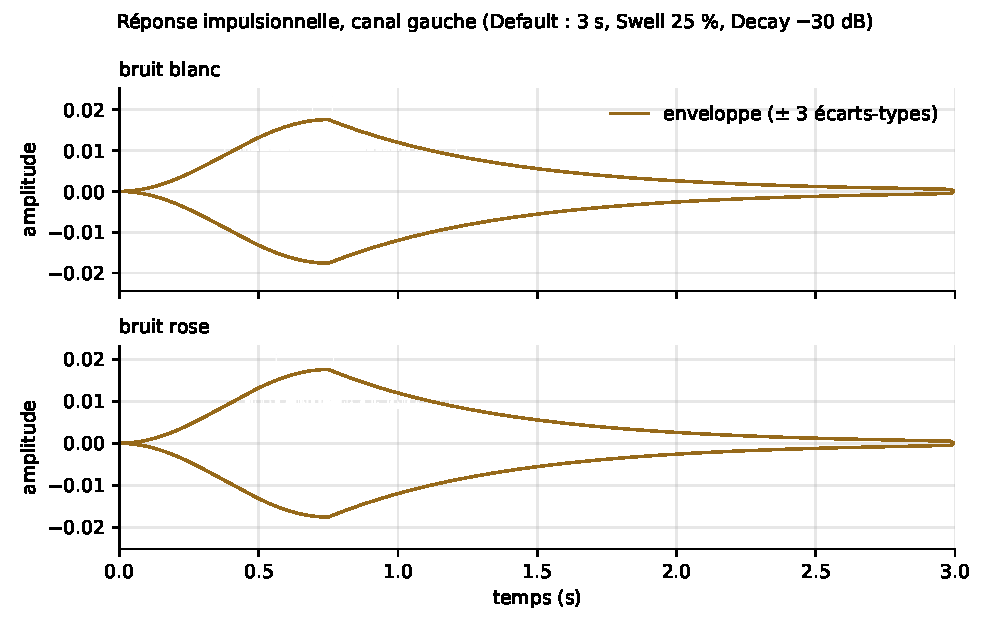
\includegraphics[width=\textwidth]{fig_reponse.pdf}
\caption{Réponse du préréglage Default, canal gauche, en bruit blanc et en bruit rose, avec son
enveloppe.}
\label{fig:reponse}
\end{figure}

\begin{figure}[htbp]
\centering
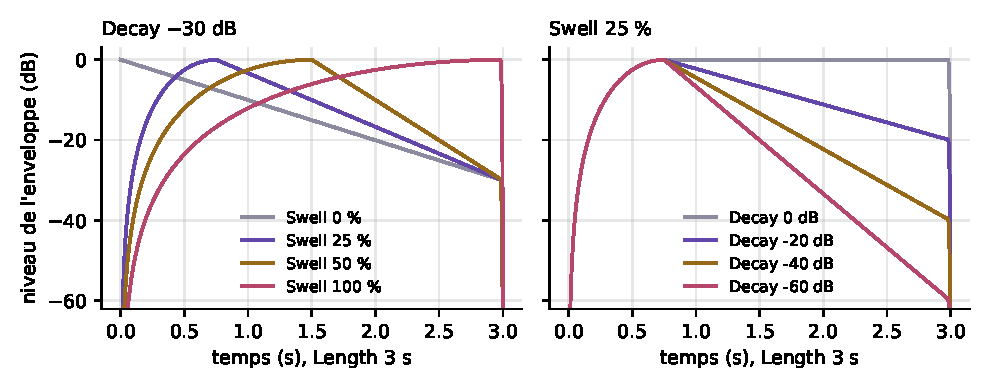
\includegraphics[width=\textwidth]{fig_enveloppes.pdf}
\caption{Enveloppe pour une longueur de 3\,s : effet de Swell (à gauche) et de Decay (à droite).}
\label{fig:enveloppes}
\end{figure}

\begin{figure}[htbp]
\centering
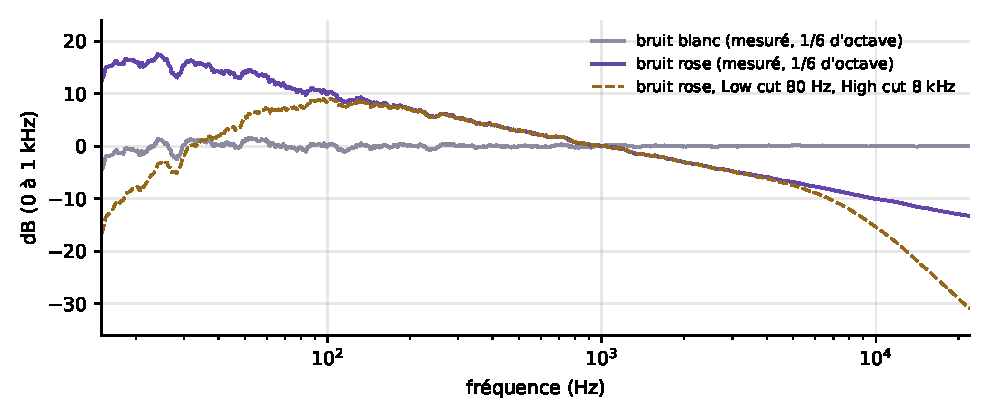
\includegraphics[width=\textwidth]{fig_spectre.pdf}
\caption{Spectre de la réponse selon Colour (moyenne des deux canaux, 4\,s, enveloppe plate),
mesuré sur les réponses du greffon et lissé au sixième d'octave ; en tirets, le bruit rose avec
Low cut 80\,Hz et High cut 8\,kHz.}
\label{fig:spectre}
\end{figure}

\begin{figure}[htbp]
\centering
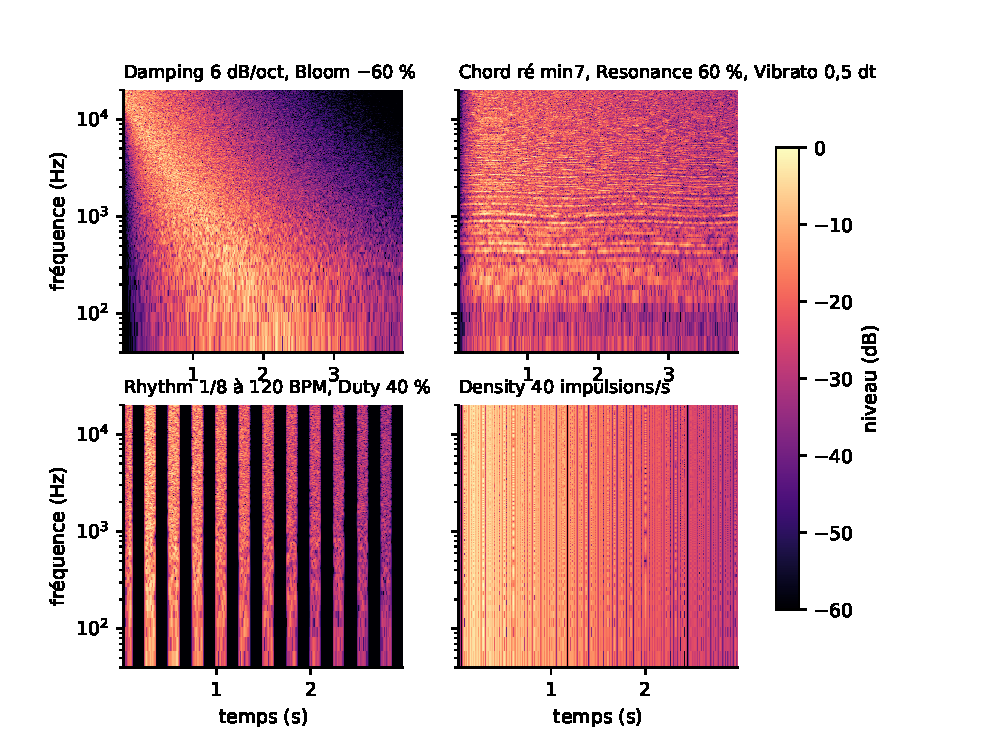
\includegraphics[width=\textwidth]{fig_traitements.pdf}
\caption{Cartes temps-fréquence de réponses du greffon (bruit blanc) : Damping et Bloom (les aigus
arrivent tôt et meurent vite), accord avec vibrato (les harmoniques des quatre notes ondulent),
porte rythmique, bruit épars (impulsions isolées).}
\label{fig:traitements}
\end{figure}

\begin{figure}[htbp]
\centering
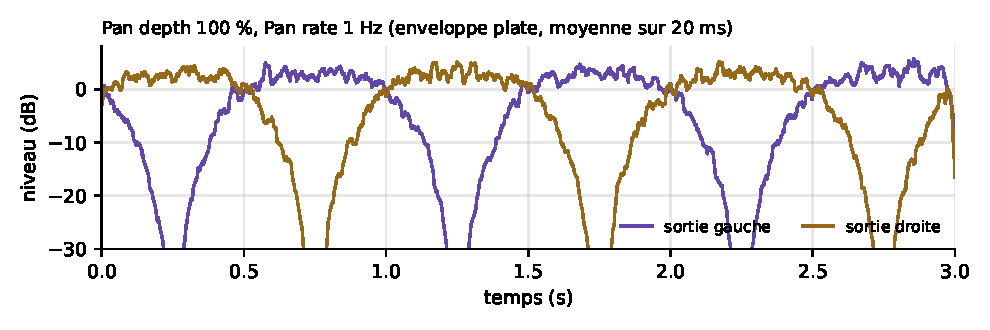
\includegraphics[width=\textwidth]{fig_stereo.pdf}
\caption{Mouvement stéréo : niveau des sorties gauche et droite le long de la réponse.}
\label{fig:stereo}
\end{figure}

\subsection{La convolution}\label{sec:convolution}

Une réponse de 10\,s à 48\,kHz compte 480\,000 échantillons : la convolution directe coûterait
près d'un milliard de multiplications par seconde et par canal. Le greffon la calcule dans le
domaine fréquentiel, par blocs (\emph{convolution partitionnée uniforme} en
recouvrement-sauvegarde, FFT réelles de pffft), en deux étages :

\begin{center}
\begin{tikzpicture}[x=0.55mm, y=1mm]
\fill[violet!25] (0,0) rectangle (32,6);
\foreach \i in {0,4,...,28} \draw[violet] (\i,0) rectangle (\i+4,6);
\fill[amber!25] (32,0) rectangle (240,6);
\foreach \i in {32,48,...,224} \draw[amber] (\i,0) rectangle (\i+16,6);
\draw[ink] (0,0) rectangle (240,6);
\node[font=\scriptsize, above] at (16,6) {tête};
\node[font=\scriptsize, above] at (136,6) {queue};
\node[font=\scriptsize, below] at (0,0) {0};
\node[font=\scriptsize, below] at (32,0) {$2M$};
\node[font=\scriptsize, below] at (240,0) {$N$};
\draw[<->] (0,-6) -- node[below, font=\scriptsize] {blocs de $B = 256$} (32,-6);
\draw[<->] (32,-6) -- node[below, font=\scriptsize] {blocs de $M$ = 4096 à 16\,384} (240,-6);
\end{tikzpicture}
\end{center}

\begin{itemize}
\item \textbf{Tête} : les $2M$ premiers échantillons de la réponse, en blocs de $B = 256$. À
  chaque bloc de 256 échantillons d'entrée : une FFT de 512 points, un produit par bloc de la
  réponse, une FFT inverse. C'est cet étage qui fixe la latence : 256 échantillons.
\item \textbf{Queue} : le reste, en blocs de $M$ = 4096 échantillons ($f_s \leq 50$\,kHz), 8192
  ($\leq 100$\,kHz) ou 16\,384. Le bloc $j$ de l'entrée n'agit sur la sortie qu'à partir de
  l'échantillon $jM + 2M$ : le greffon a donc $M$ échantillons de temps pour calculer sa
  contribution (une FFT, les produits avec tous les blocs de la queue, une FFT inverse) et la
  répartit également sur les $M/B$ blocs de 256 qui précèdent. Il n'y a ni pointe de calcul ni
  fil supplémentaire dans le traitement audio.
\end{itemize}
Les deux étages partagent les spectres de l'entrée déjà calculés (lignes à retard fréquentielles) ;
avec Cross, chaque sortie ajoute les produits des réponses croisées par les spectres de l'autre
entrée, ce qui double les produits sans transformée de plus.
Le résultat est celui de la convolution exacte, aux arrondis du calcul en simple précision près :
les tests le comparent à une convolution directe en double précision, avec un écart d'au plus
$4{,}4 \cdot 10^{-7}$ de la crête, pour des réponses de 1 échantillon à $5M$ et à 48, 96 et
192\,kHz, et de $3{,}5 \cdot 10^{-7}$ avec les réponses croisées.

\paragraph{Coût.} Mesuré sur un cœur (blocs de 256, stéréo) :
\begin{center}
\small
\begin{tabular}{@{}l r r r@{}}
\toprule
Length & 48\,kHz & 96\,kHz & 192\,kHz \\
\midrule
3\,s  & 1,0\,\% & 3,0\,\% & 8,8\,\% \\
10\,s & 2,2\,\% & 5,4\,\% & 15\,\% \\
10\,s, Cross & 4,5\,\% & 10\,\% & 25\,\% \\
\bottomrule
\end{tabular}
\end{center}
Les traitements du bruit ne coûtent rien pendant la lecture : ils sont dans la réponse. La mémoire
occupée est de l'ordre de 20\,Mo à 48\,kHz (40\,Mo avec Cross) ; pendant une reconstruction, le
calcul de la réponse en demande davantage, brièvement (jusqu'à 340\,Mo dans le pire cas à
192\,kHz).

\subsection{Changement de réponse}\label{sec:changement}

Les réglages des sections SOURCE, TUNE, ENVELOPE et MOTION définissent la réponse : en changer
un oblige à la refaire, de même qu'un changement du tempo de l'hôte quand RHYTHM est actif. Un
réglage sans effet avec les autres (NOTE quand TUNE est sur OFF, par exemple) ne la refait pas.
Ce travail est fait dans un fil du greffon, jamais dans le traitement audio, qui continue avec
l'ancienne réponse. Quand la nouvelle est prête, elle est prise au début d'un bloc de queue.
Comme les spectres de l'entrée ne dépendent pas de la réponse, la nouvelle réponse dispose
d'emblée de tout le passé du signal : le pad ne repart pas de zéro. La sortie passe de l'ancienne
réponse à la nouvelle par un fondu linéaire de $M$ échantillons (85\,ms à 48\,kHz), puis
l'ancienne est libérée, dans le fil du greffon.

Tourner un de ces boutons pendant la lecture donne donc une suite de fondus, sans clic, avec un
léger retard. À l'activation du greffon (début de lecture ou de rendu), la réponse est construite
sur-le-champ : un rendu commence toujours avec la bonne réponse.

\subsection{Pré-retard, largeur, filtres, mélange et sortie}

\paragraph{Pre-delay.} Retard entier en échantillons du pad, juste après la convolution ; un
changement passe de l'ancien retard au nouveau par un fondu de 30\,ms, le suivant attend la fin
du fondu.

\paragraph{Filtres.} Low cut et High cut sont des filtres de Butterworth du second ordre (formules
de Robert Bristow-Johnson), en double précision ; leur fréquence est limitée à 0,45\,$f_s$. Au
neutre, leurs coefficients sont ceux de l'identité : la sortie est alors exactement l'entrée.

\paragraph{Width.} Sur le pad : $m = (p_L + p_R)/2$, $s = (p_L - p_R)/2 \cdot$ Width,
$p_L' = m + s$, $p_R' = m - s$.

\begin{figure}[htbp]
\centering
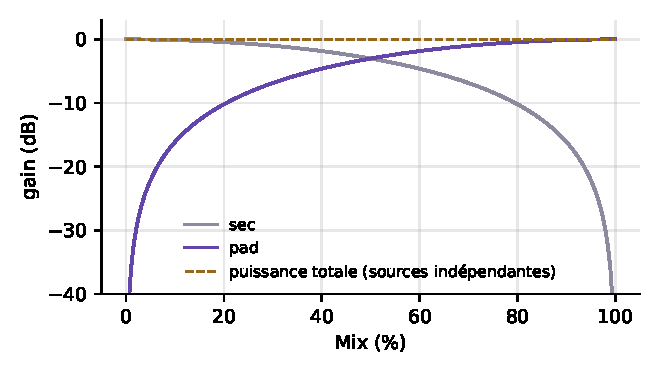
\includegraphics[width=0.6\textwidth]{fig_mix.pdf}
\caption{Loi du mélange : gains du sec et du pad en fonction de Mix.}
\label{fig:mix}
\end{figure}

\paragraph{Mélange et sortie.} $y = (\text{pad} \cdot \sin(\tfrac{\pi}{2} m) + \text{sec retardé}
\cdot \cos(\tfrac{\pi}{2} m)) \cdot g$, $g$ = gain de Output ; les gains valent exactement 0 et
1 aux deux bouts de Mix.

\subsection{Lissage des réglages et Bypass}\label{sec:lissage}

Mix, Width, Output et les coefficients des deux filtres vont linéairement à leur nouvelle valeur
en 20\,ms, puis la prennent exactement : pas de crépitement quand on les tourne ou les automatise.
Les réglages de la réponse changent par fondu (section~\ref{sec:changement}).

\paragraph{Bypass.} La sortie devient le sec retardé de 256 échantillons, exactement, par un fondu
de 10\,ms ; la latence reste la même. La convolution continue de tourner pendant le Bypass, si
bien que le pad est déjà là quand on le relâche.

\subsection{Nombres dénormaux}

Dans un silence, les états des filtres décroissent vers zéro et passeraient par les nombres
dénormaux, très lents sur x86. Le greffon active les modes FTZ/DAZ du processeur le temps de son
calcul et rend à l'hôte son propre état en sortie.

% ==============================================================================================
\section{Conseils d'utilisation}

\begin{description}
\item[Nappe à partir d'un instrument.] Soft pad ou Endless wash en départ auxiliaire, Mix à
  100\,\% : des notes jouées détaché deviennent un fond continu. Plus Length est long et Decay
  proche de 0, plus la nappe est stable.
\item[Nappe accordée.] Tuned drone ou Chord pad sur une source riche (batterie, bruit, guitare
  saturée) : la nappe prend la note ou l'accord. Accorder NOTE sur la tonalité du morceau ; monter
  RESONANCE pour des notes plus nettes.
\item[Épaissir.] Short smear (0,4\,s) sur une voix, une guitare ou une caisse claire : le son
  gagne une queue dense, sans l'espace d'une réverbération.
\item[Montées.] Reverse swell : chaque attaque monte pendant 2\,s puis s'arrête net. Avec un
  départ placé quelques temps avant, la montée précède le son.
\item[Rythme.] Pulse gate : la nappe pulse en croches au tempo ; DUTY court pour des échos
  rythmés, long pour une respiration.
\item[Réalisme.] DAMPING 3 à 6\dB/oct rend la queue plus naturelle ; BLOOM négatif donne une
  nappe qui se réchauffe en s'installant.
\item[Grave.] Les bruits rose et brun donnent beaucoup de grave : Low cut 60 à 150\,Hz, surtout en
  départ sur plusieurs pistes.
\item[Souffle.] Un bruit blanc ou bleu fait entendre un souffle sur les sons doux : High cut entre
  6 et 12\,kHz, ou une couleur plus basse.
\item[Texture.] Si une fréquence ressort trop sur un son tenu, changer Seed.
\item[Mono.] Le pad est très large ; vérifier en mono et réduire Width si le mixage se creuse.
\item[Comparer deux réglages.] Régler A, copier vers B (\ctl{A>B}), modifier B, puis basculer A
  | B.
\end{description}

\section{Fichiers, projets et compatibilité}\label{sec:fichiers}

\begin{description}
\item[Avec le projet.] Tous les réglages et le jeu A/B inactif (état \texttt{ab}). Les réglages
  sont relus par leur nom : ajouter un réglage dans une version future ne casse pas un projet. La
  réponse n'est pas enregistrée : elle est refaite à l'identique à partir des réglages.
\item[Sur l'ordinateur.] Le thème dans \texttt{padifier.conf} (\texttt{theme=dusk} ou
  \texttt{pearl}) et vos préréglages dans \texttt{presets/}, un fichier \texttt{<nom>.preset}
  chacun, dans le dossier :
  \begin{itemize}
  \item Windows : \verb|%APPDATA%\Padifier\| ;
  \item Linux : \verb|$XDG_CONFIG_HOME/padifier/|, à défaut \verb|~/.config/padifier/|.
  \end{itemize}
\item[Format d'un préréglage.] Texte, une ligne \texttt{clé=valeur} par réglage (les symboles
  des paramètres : \texttt{colour}, \texttt{length}, \texttt{swell}, \texttt{decay},
  \texttt{seed}, \texttt{density}, \texttt{tune}, \texttt{note}, \texttt{chord},
  \texttt{resonance}, \texttt{damping}, \texttt{bloom}, \texttt{lforate}, \texttt{lfopitch},
  \texttt{lfotone}, \texttt{rhythm}, \texttt{duty}, \texttt{panrate}, \texttt{pandepth},
  \texttt{cross}, \texttt{predelay}, \texttt{lowcut}, \texttt{highcut}, \texttt{width},
  \texttt{mix}, \texttt{output}), nombres avec un point décimal quelle que soit la langue du
  système. Une clé absente prend sa valeur par défaut, une valeur hors bornes est ramenée dans les
  bornes, une ligne inconnue est ignorée. Copier le fichier suffit à partager un préréglage.
\item[Depuis la 1.0.] Le réglage Noise (blanc ou rose) est devenu Colour : un projet ou un
  préréglage de la 1.0 garde ses autres réglages, la couleur revient au rose ($-3$) et les
  nouveaux réglages à leur défaut, si bien que le son est celui de la 1.0 en bruit rose.
\end{description}

% ==============================================================================================
\section{Limites connues}\label{sec:limites}
\begin{itemize}
\item Latence de 256 échantillons : compensée par l'hôte, mais audible si l'on joue en direct à
  travers le greffon avec un très petit tampon.
\item Un changement des réglages de la réponse arrive avec un léger retard (le temps de la refaire,
  jusqu'à 1\,s dans le pire cas à 192\,kHz) ; en rendu hors ligne plus rapide que le temps réel,
  une automatisation de ces réglages peut donc tomber un peu plus tard qu'à la lecture.
\item Les mouvements (LFO, rythme, stéréo) partent de l'attaque de chaque son, pas du temps du
  morceau.
\item La convolution ne crée pas de fréquence : TUNE fait ressortir ce que la source contient près
  des notes, il ne transpose rien.
\item Le pad n'a pas de gel (\emph{freeze}) : il suit toujours l'entrée.
\item La saisie au clavier (valeurs, noms de préréglages) dépend de l'hôte : certains gardent le
  clavier pour eux.
\item L'hôte ne voit que les préréglages d'usine.
\end{itemize}

% ==============================================================================================
\section{Crédits}
FFT : pffft, Julien Pommier, d'après FFTPACK (Paul Swarztrauber, NCAR). Générateur
pseudo-aléatoire : SplitMix64 (Steele, Lea et Flood, 2014). Filtres : formules de Robert
Bristow-Johnson (\emph{Audio EQ Cookbook}). Cadre de greffon et interface : DPF (DISTRHO Plugin
Framework, ISC), avec NanoVG (zlib), pugl (ISC), les en-têtes CLAP (MIT) et la police DejaVu Sans.
Les notices de licence de ces composants sont dans \texttt{THIRD\_PARTY\_LICENSES.txt}, installé
avec le greffon et joint à chaque archive.

\end{document}
